% 为使用bibliography参考文献,编译选项选xelatex-bibtex-xelatex*,但很慢
% 不是最终版本,可以只选xelatex

% 本模板由松鼠制作
% github地址:github.com/Sciurus365/PhysChemLab
% 2018年1月23日

%推荐在编辑器窗口使用consolas+微软雅黑混合字体码代码==


\RequirePackage[l2tabu, orthodox]{nag}
\documentclass[UTF8]{article}


\usepackage{threeparttable}
\usepackage[zihao=-4]{ctex}
\usepackage{graphicx}
\usepackage{multicol}
\usepackage[a4paper]{geometry}
\usepackage{booktabs}
\usepackage{microtype}
\usepackage{siunitx}
\usepackage{ragged2e}
\usepackage{fontspec}
\usepackage{multirow}
\usepackage{mhchem}
\usepackage[square,sort,comma,numbers,super]{natbib}
\usepackage{fancyhdr}
\usepackage{url}

\usepackage{amsmath}%输入特殊数学符号
\usepackage{float}%浮动体控制
\usepackage[figuresright]{rotating}%竖排表格


% 纸张、页边距设置
\graphicspath{{figures/}}
\geometry{left=2.0cm,right=2.0cm,top=2.0cm,bottom=2.0cm}

% 统一全文英语字体
\usepackage{unicode-math}
\setmathfont{XITS Math}
%\setmainfont{Times New Roman}
\setmainfont{XITS Math}


% 实验相关信息设置
\newcommand{\expname}{中级物理化学实验报告}
\newcommand{\expdate}{日期}
\newcommand{\exptemperature}{0}
\newcommand{\exppressure}{0}
\newcommand{\expteacher}{指导教师}



% 页眉页脚设置
\pagestyle{fancy}  
\lhead{拉曼光谱仪搭建与应用}  
\chead{\expname}  
\rhead{\expdate}  
\lfoot{}  
\cfoot{\thepage}  
\rfoot{}  
\renewcommand{\headrulewidth}{0.4pt}  
\renewcommand{\footrulewidth}{0.4pt}  

% 温度 电动势 浓度和气压的快速输入
\newcommand{\swd}[1]{\SI{#1}{\degreeCelsius}}
\newcommand{\sdds}[1]{\SI{#1}{\volt}}
\newcommand{\snd}[1]{\SI{#1}{\mole \per \liter}}
\newcommand{\sqy}[1]{\SI{#1}{\kilo \pascal}}
% 摄氏度、公式中文本、\varepsilon的快速输入
% \newcommand{\dC}{\si{\degreeCelsius}}
\newcommand{\tr}[1]{\textrm{#1}}
\newcommand{\ve}{\varepsilon}

\def\dC{\si{\degreeCelsius}}
\def\kPa{\,\si{kPa}}
\newcommand{\dw}[1]{\,\mathrm{#1}}

\def\d{\mathrm{d}}
\def\e{\mathrm{e}}
\def\i{\mathrm{i}}
\def\p{\partial}
\def\toinfty{\to \infty}


% 如果需要在三线表中插入竖线,请进行以下设置以避免竖线被割断
%\belowrulesep=0ex
%\aboverulesep=0ex

% 使用siunitx包报告不确定度时,以下设置可以使结果以\bar(X) \pm \sigma 的形式表示
% 使用siunitx包书写单位时,以下设置可以使单位之间加\cdot点
\sisetup{
	separate-uncertainty = true,
	inter-unit-product = \ensuremath{{}\cdot{}}
}

\begin{document}
	
	%——————————封面页——————————
	\begin{titlepage}
		\vspace*{1cm}
		\begin{figure}[h]
			\centering
			
\includegraphics[width=0.7\linewidth]{logo}
		\end{figure}
		
		\vspace*{0.5cm}
		
		\begin{center}
			\Huge{\textbf{拉曼光谱仪搭建与应用}}
			
			\Large{\expname}
		\end{center}
		
		\vspace*{0.5cm}
		
		\begin{table}[h]
			\centering
				\begin{tabular}{cccc}
					元培学院 & 肖舒凡 \\
					化学与分子工程学院  & 曾志炜 \\
					化学与分子工程学院  & 傅洪鑫 \\
				\end{tabular}
		\end{table}
	
	\vspace*{1cm}
	
	\textbf{摘要}\quad  晚点再写
	
	\end{titlepage}
	
	\normalsize

	\section{引言}
	拉曼光谱是一种分析材料结构和化学成分的有效手段。拉曼光谱基于光的非弹性散射,广泛应用于材料科学、生物医学、环境监测等领域。本实验的目标是搭建自制的拉曼光谱仪,并探索其原理和应用。
	

	\section{基本原理}
	\subsection{拉曼散射原理}
	单色光通过透明介质,在透射和反射方向以外出现的光,即为散射光。散射的粒子为分子大小时,发生Rayleigh散射,其频率与入射光相同。1928年,印度物理学家C.V.Raman发现频率与入射光不同的散射光,称为Raman散射,其中频率较低的称为Stokes散射,频率较高的称为Anti-Stokes散射。
	
	量子理论的解释如图\ref{Raman}\footnote{source \url{https://en.wikipedia.org/wiki/Raman_scattering}},分子某一化学键的振动能级吸收光子,从基态受激跃迁至虚态,再跃迁至激发态并放出较低能量的光子,即为Stokes散射过程,而从激发态跃迁至虚态,再跃迁至基态,放出较高能量的光子,即为Anti-Stokes散射过程。按Boltzmann统计,处于振动基态的分子远远多于处于振动激发态的分子,因此Stokes散射的强度较Anti-Stokes散射强得多。Raman散射过程中的频率位移与入射光频率无关,因此以Stokes散射强度对频率位移作图,得到物质分子的拉曼光谱。
	\begin{figure}[htp]
		\centering
		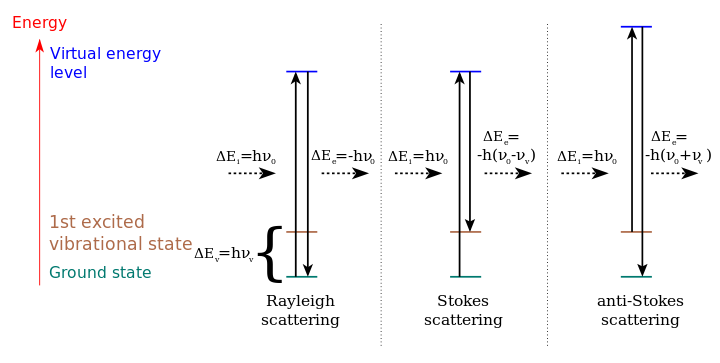
\includegraphics[width=0.9\linewidth]{figures/Ramanscattering.png}
		\caption{拉曼散射的量子理论解释} \label{Raman}
	\end{figure}

	\subsection{表面增强拉曼光谱原理}
	这里简单介绍表面增强的原理


	\section{软件开发}
	拉曼光谱仪数据采集及自动分析软件使用LabView自主开发,配套硬件为CCD及数据传输线。主要实现以下功能:
	\begin{itemize}
		\item 自动采集:软件自动采集数据、绘制及更新拉曼光谱图。
		\item 设置积分时间:软件支持可变积分时间,可手动设置强度对应的积分时间。
		\item 采集暗背景:软件支持手动采集暗背景,并在实验中自动扣除。
		\item 自动寻峰标定:软件支持基准物质自动寻峰标定、曲线拟合、结果转换一键完成。
		\item 图像转换:软件支持强度-像素图、强度-拉曼位移图之间的任意转换。
		\item 数据导出:软件支持以表格或图片形式导出数据。
	\end{itemize}
	软件本体、工程文件及使用文档详见github项目 
	\begin{itemize}
		\item \url{https://github.com/22w1006/Raman-Spectroscopy-Assistant}。
	\end{itemize}
	
	
	
	\section{实验步骤}	
	\subsection{实验用品}
	\textbf{元件} \quad 532 nm 激光器,Semrock 二向色镜,10 X 物镜,样品池架,平面镜,Edge 滤光片,凸透镜,狭缝,凹面镜,光栅( 25 mm $\times$ 25 mm $\times$ 6 mm, Blaze Wavelength 500 nm, Grooves 1200/mm, Blaze Angle  $17°27'$ ),CCD检测器。光学元件架,光学支杆套件,遮光器材。

	\begin{figure}[htp]
		\centering
		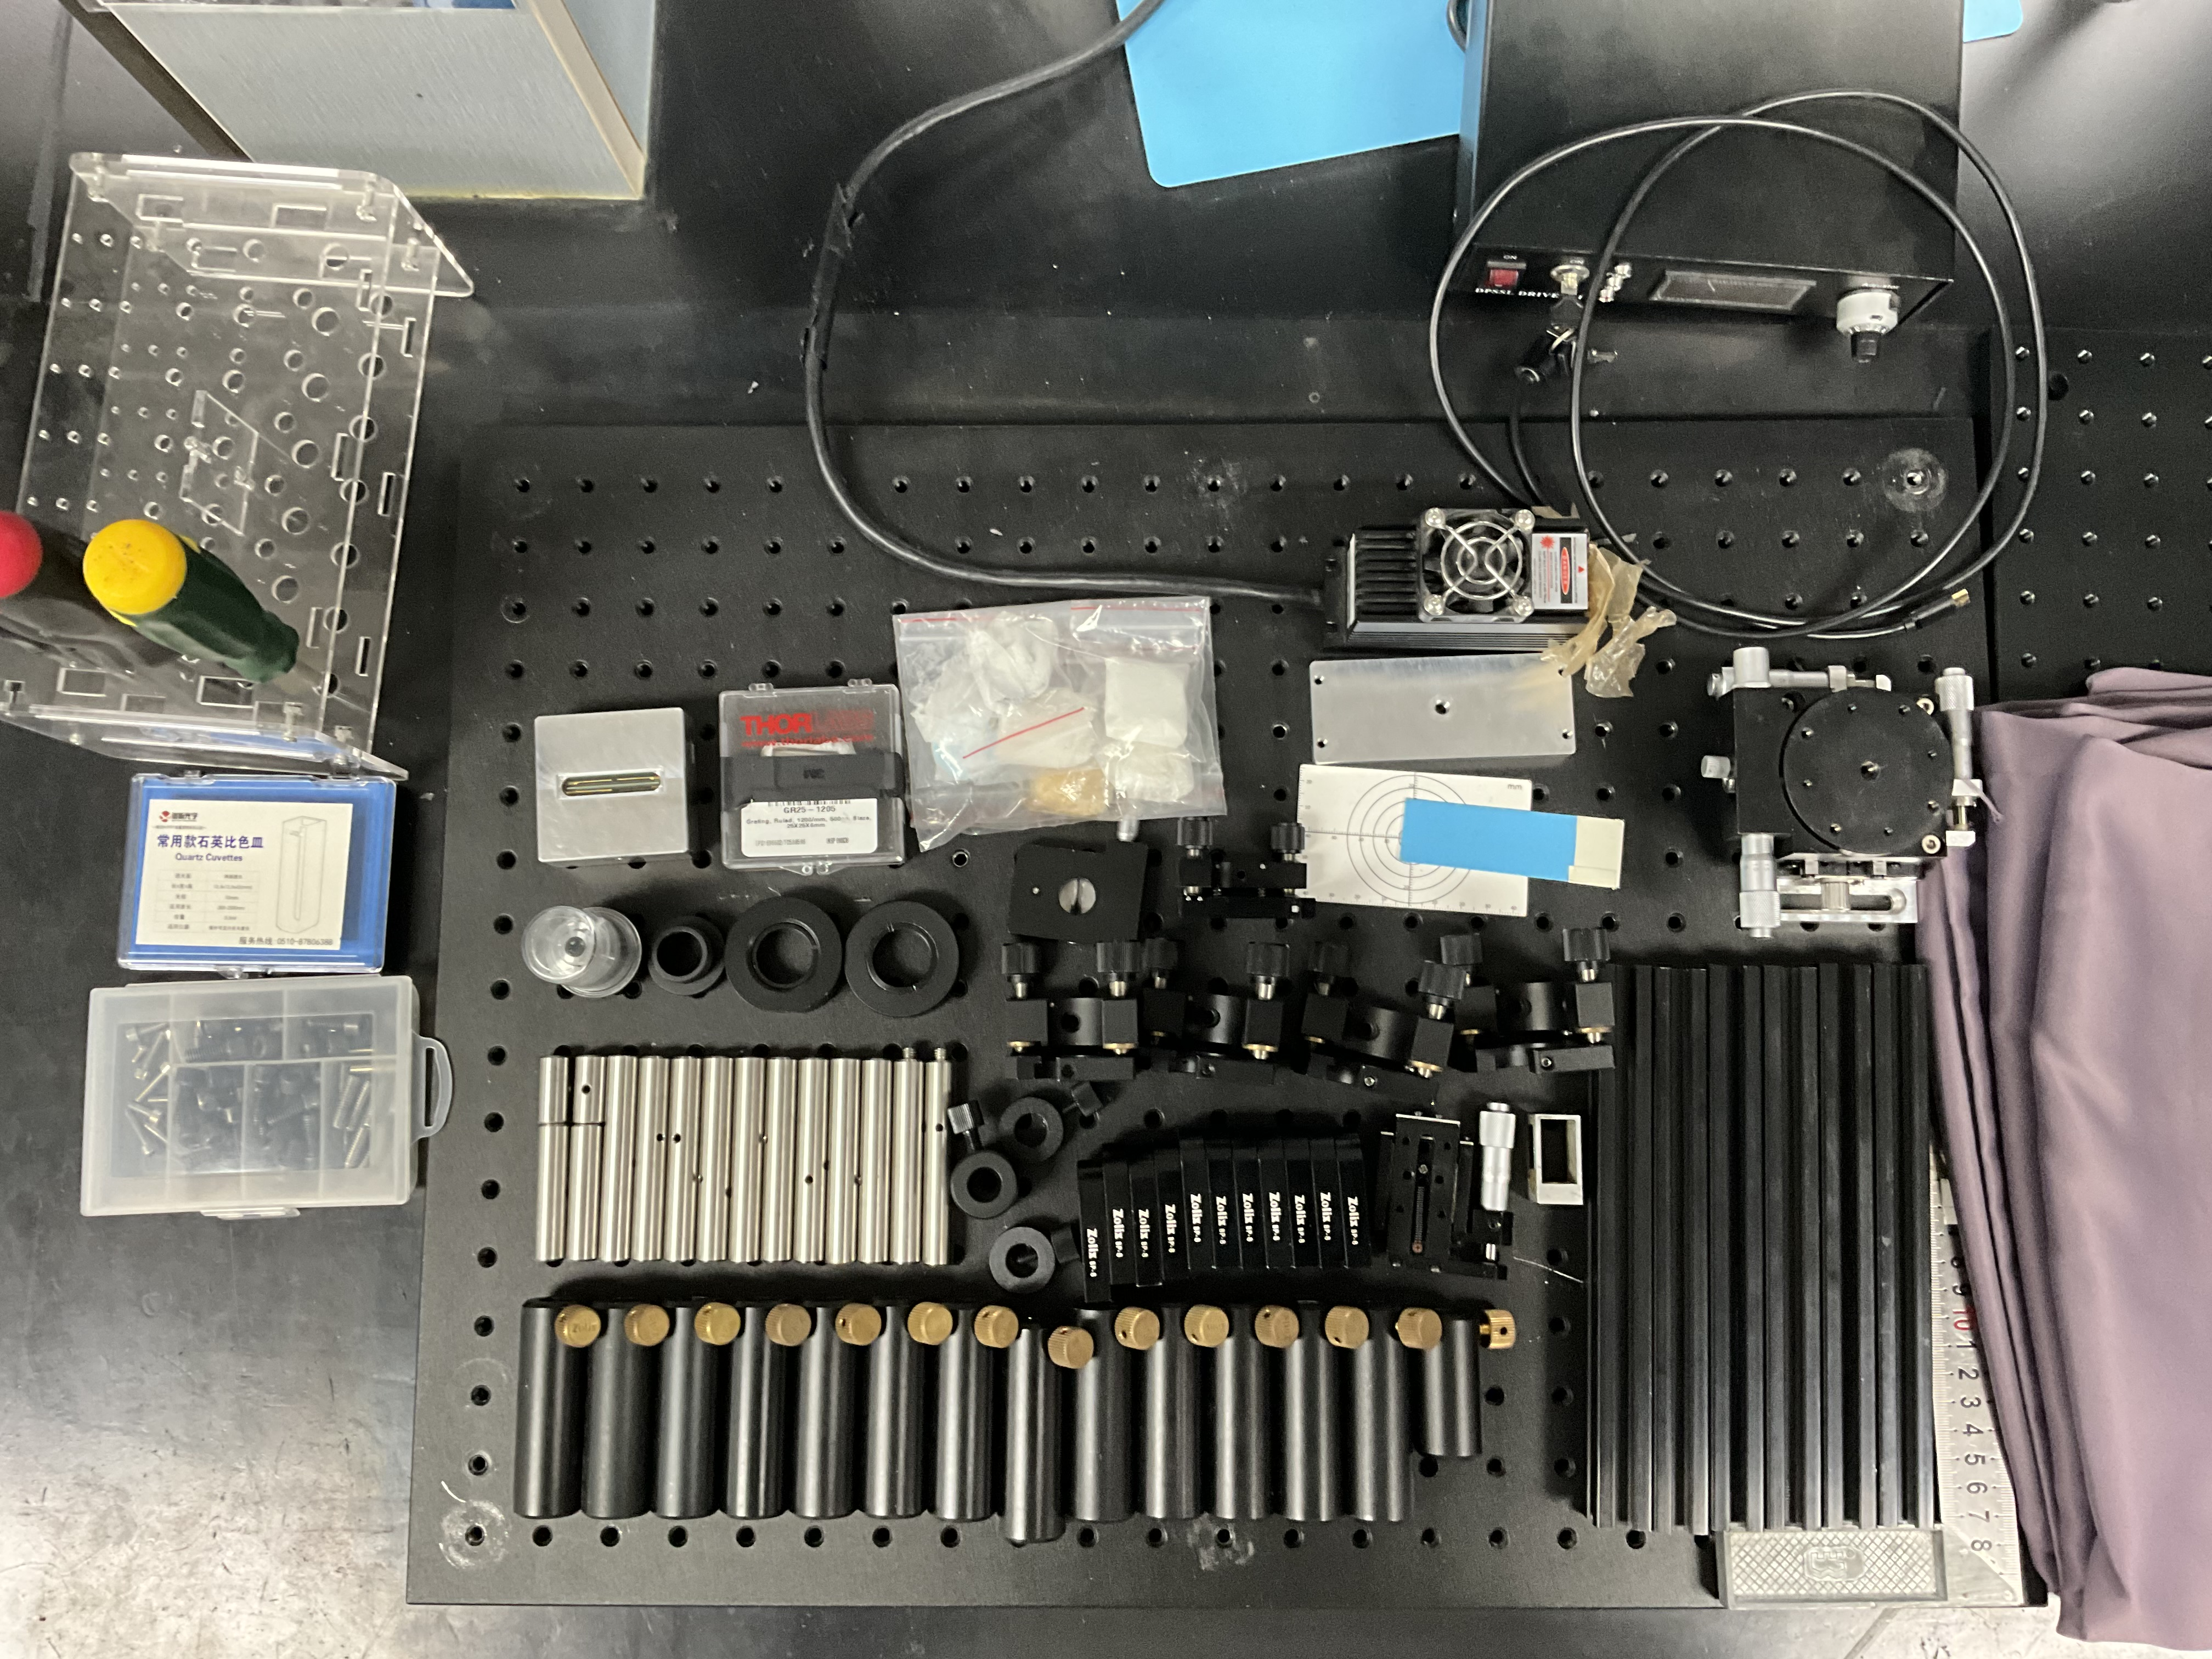
\includegraphics[width=0.5\linewidth]{figures/IMG_0014.JPG}
		\caption{仪器元件展示} \label{}
	\end{figure}
	
	\textbf{试剂} \quad 乙醇,丙酮。1-己胺,苯胺,对硝基苯胺。【表面增强相关试剂】。无水硫酸钠,重水。
	
	\textbf{仪器} \quad 分析天平,移液枪,电磁搅拌器,离心机,超声机等【表面增强相关仪器】。直流稳压电源,铂电极。

	\subsection{拉曼光谱仪的搭建、标定与测试}
	根据原理图搭建拉曼光谱如图\ref{instrument}。仪器有配套的自行裁剪的挡板外壳,以及测量时遮光用的布料。
	\begin{figure}[htp]
		\begin{minipage}[t]{0.5\textwidth}
			\centering
			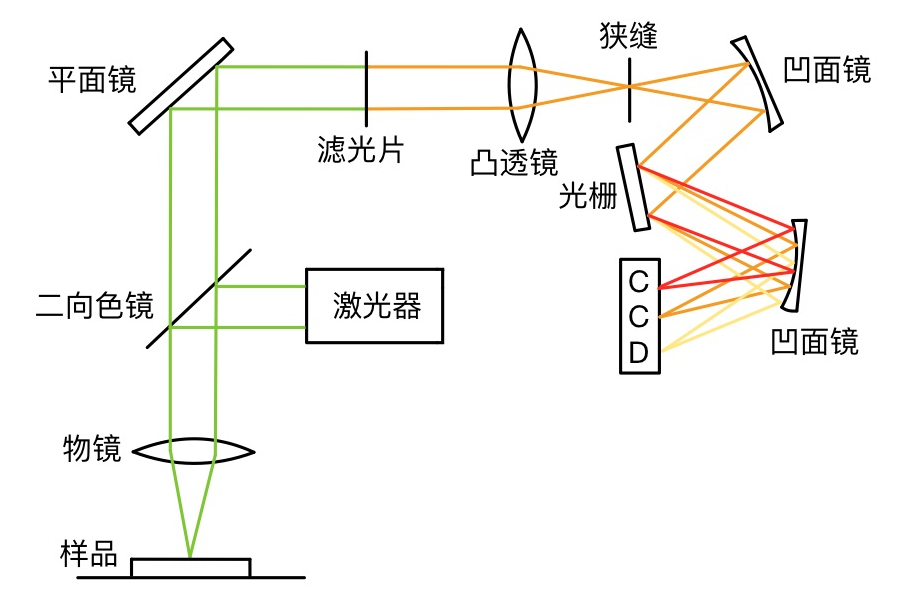
\includegraphics[width=\linewidth]{figures/construction.png} 
		\end{minipage}
		\begin{minipage}[t]{0.5\textwidth}
			\centering
			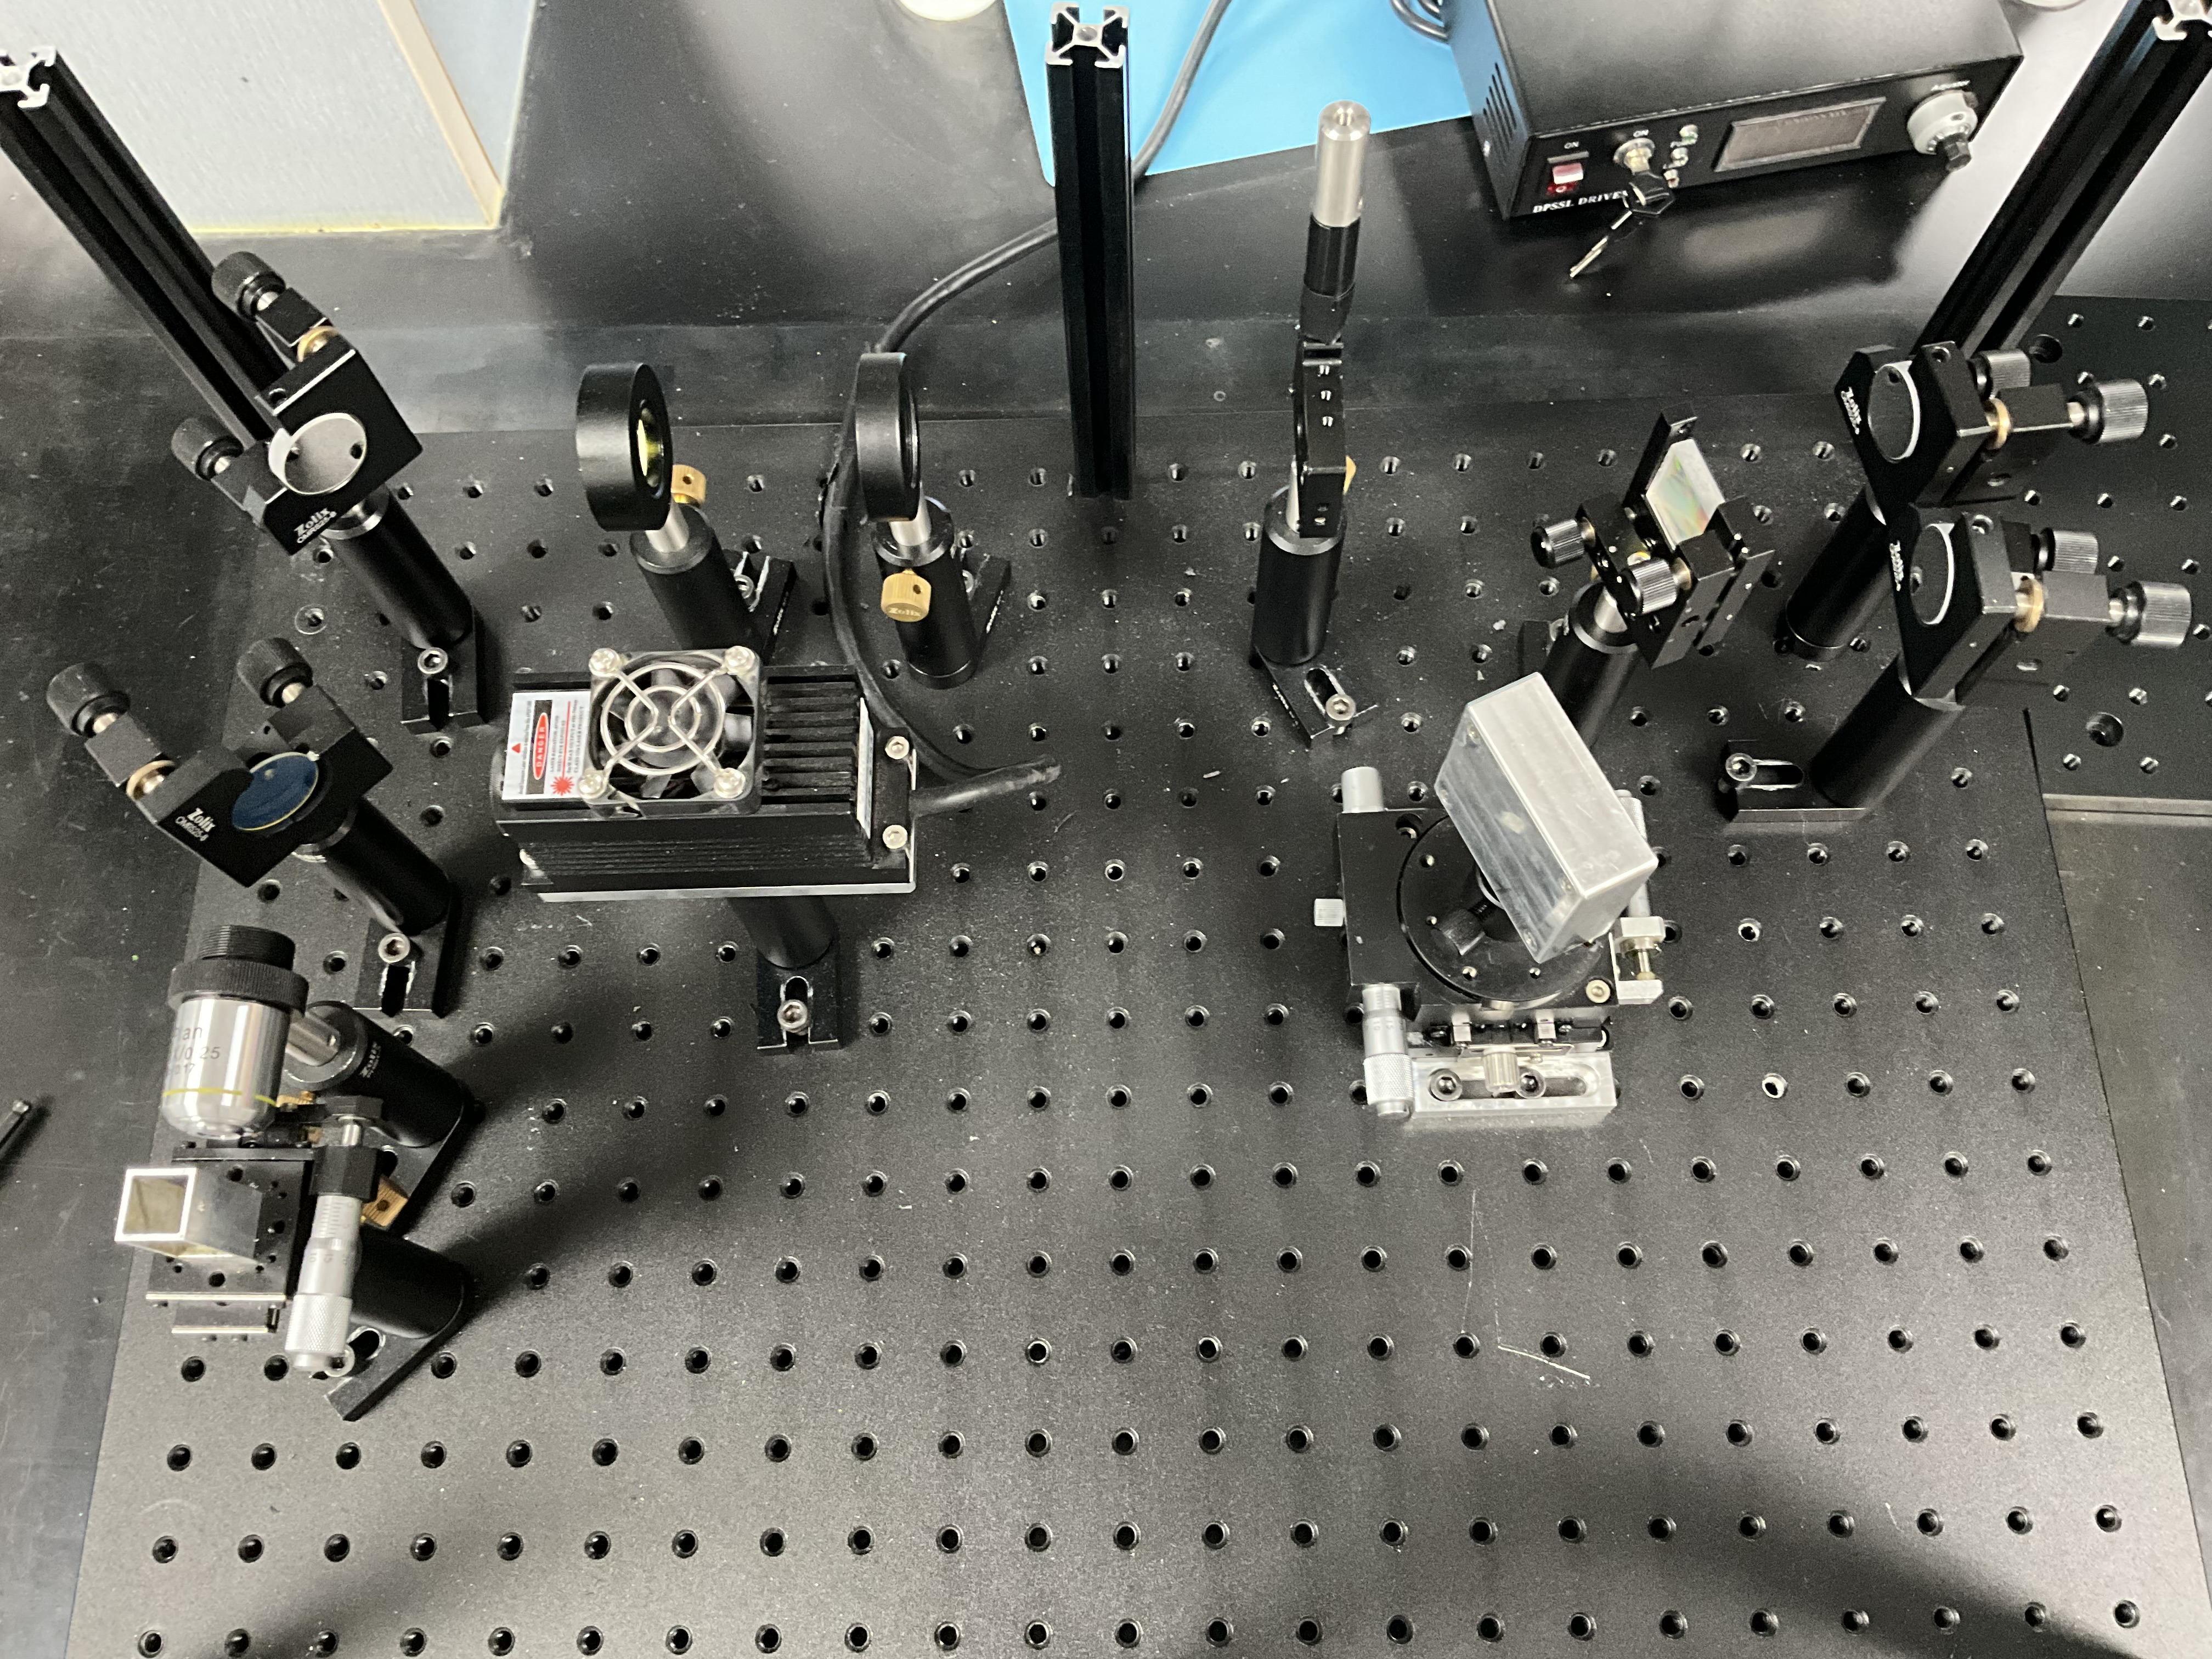
\includegraphics[width=\textwidth]{figures/IMG_0008.JPG}
		\end{minipage}
		\caption{仪器原理与内部构造} \label{instrument}
	\end{figure}

	\textbf{软件准备}\quad 打开软件“拉曼数据助手”,选择合适的CCD检测器串口。点击【开始采集】按键,应能在左侧窗口中观察到仪器的暗背景信号。调节合适的积分时间,例如 5 s,暗背景信号的强度将随之变化。点击【采集暗背景】按键。等待一段时间,应略长于积分时间。再次点击【采集暗背景】按键,结束采集。随后,再点击【扣除暗背景】按键,软件准备完毕。
	
	\textbf{仪器标定}\quad 打开激光光源,功率设置为 $1 \dw{W}$ 左右。测定乙醇光谱图,用以标定仪器。谱图稳定后,点击【自动寻峰】按键,用乙醇的七个峰对应像素的位置显示在窗口右侧。选择下方坐标轴选项,将横坐标变换为波数。观察到标定拟合 $r^2>0.9999$,窗口左侧变换为乙醇的拉曼光谱图,标定完成。

	\textbf{样品测试}\quad 放入待测样品,软件中出现样品的拉曼光谱数据,可以保存为图像或表格进行后续处理。

	\subsection{纳米银溶胶的制备}

	\subsection{样品测试}
	\subsubsection{测试1:己胺、苯胺、对硝基苯胺}
	己胺和苯胺为液体,直接测定各自的拉曼光谱。对硝基苯胺为固体,测定其的丙酮溶液,并将丙酮的背景信号扣除,得到拉曼光谱。

	\subsubsection{测试2:表面增强}

	\subsubsection{测试3:水和重水}
	移取400 $\dw{\mu L}$ 去离子水和 400 $\dw{\mu L}$ 重水于小电解池中,加入适量无水硫酸钠,振荡溶解。测定溶液的拉曼光谱。0.25 A 恒流电解30 min,冷却后测定溶液拉曼光谱。
	
	\section{实验结果与数据分析}
	\subsection{光谱仪性能表征}
	拉曼光谱仪以乙醇的拉曼光谱为标准进行标定,依次为标准表征仪器参数和性能。测得乙醇的拉曼光谱如图。
	\begin{figure}[htp]
		\centering
		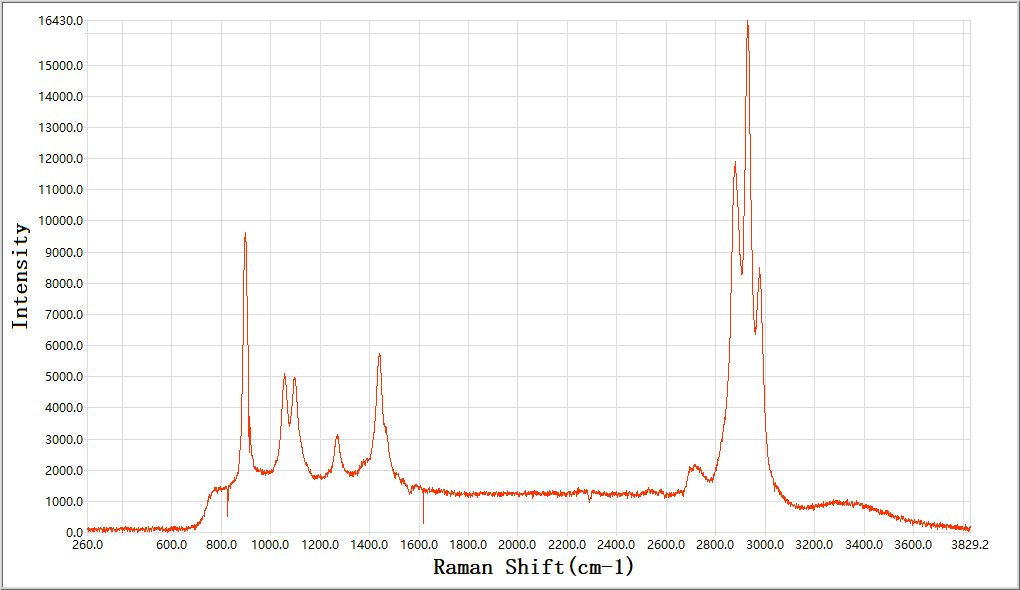
\includegraphics[width=0.8\linewidth]{figures/乙醇.png}
		\caption{乙醇的拉曼光谱} \label{ethanol}
	\end{figure}

	搭建的光谱仪具有如下特点:	
	\begin{itemize}
		\item 测量范围广:$800 \sim 3829 \dw{cm^{-1}}$,能覆盖水的远红外拉曼吸收峰。
		\item 信噪比高:用于标定的七个乙醇谱峰,信噪比如表\ref{SNR},都在 $10^2$ 的数量级。
		\item 分辨率高:乙醇在898 nm的谱峰的FWHM约为21 $\dw{cm^{-1}}$,用于标定的七个乙醇谱峰整体清晰可见,1058 $\dw{cm^{-1}}$ 和1100$\dw{cm^{-1}}$处的双峰,以及2878$\dw{cm^{-1}}$、2929$\dw{cm^{-1}}$、2976$\dw{cm^{-1}}$处的三峰,均能明显辨别。
	\end{itemize}

	\begin{table}[htp]
		\centering
		\begin{threeparttable}
			\caption{信噪比}\label{SNR}
			\small %表格内容字号小一号
			\begin{tabular} {ccccccccccccc}
				\toprule
				Raman Shift / $\dw{cm^{-1}}$ & 898 & 1058 & 1100 & 1440 & 2878 & 2929 & 2976 \\
				\midrule
				Intensity & 10242 & 5408 & 5214 & 6124 & 12622 & 17522 & 9126 \\
				estimated SNR & 211 & 97 & 92 & 114 & 267 & 383 & 185 \\
				\bottomrule
			\end{tabular}
		\end{threeparttable}
	\end{table}
	
	\subsubsection{部分测试样品的拉曼光谱结果}
	丙酮、1-己胺、苯胺、对硝基苯胺的光谱拉曼光谱如图。其中,丙酮、1-己胺、苯胺的谱图在忽略基线时与标准谱图一致,3000 $\dw{cm^{-1}}$ 附近的强峰是\ce{C-H}的振动峰。1-己胺和苯胺在3300 $\sim$ 3400 $\dw{cm^{-1}}$ 附近,强度较弱的峰是\ce{N-H}的振动峰。另外,苯胺的基线以及对硝基苯胺的异常谱图,很可能是由物质的荧光引起的,需要更换不同的激光波长来消除干扰。

	\begin{figure}[htp]
		\begin{minipage}[t]{0.5\textwidth}
			\centering
			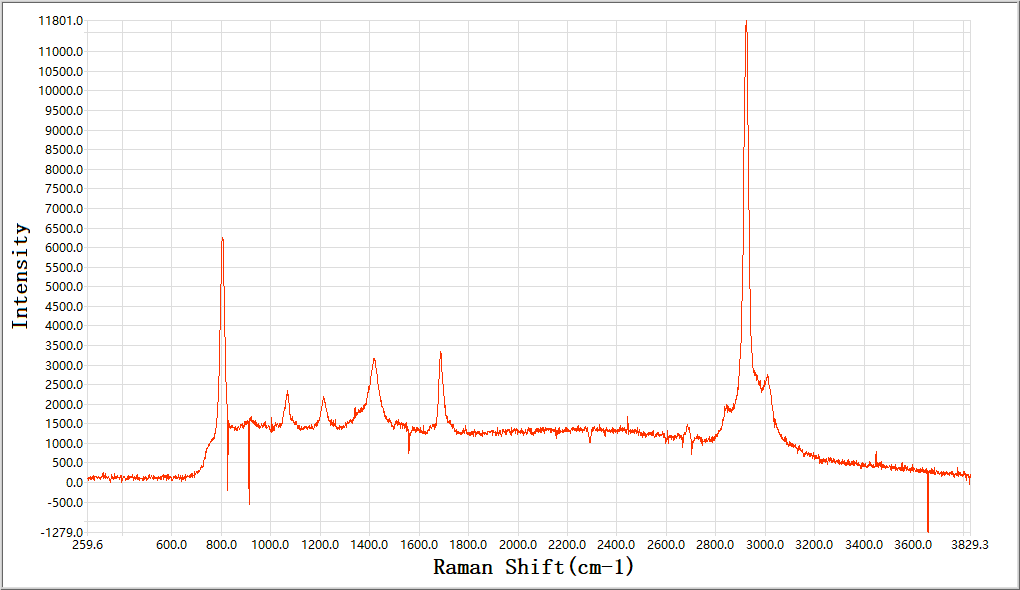
\includegraphics[width=\linewidth]{figures/丙酮.png} 
			\caption{丙酮的拉曼光谱} \label{}
		\end{minipage}
		\begin{minipage}[t]{0.5\textwidth}
			\centering
			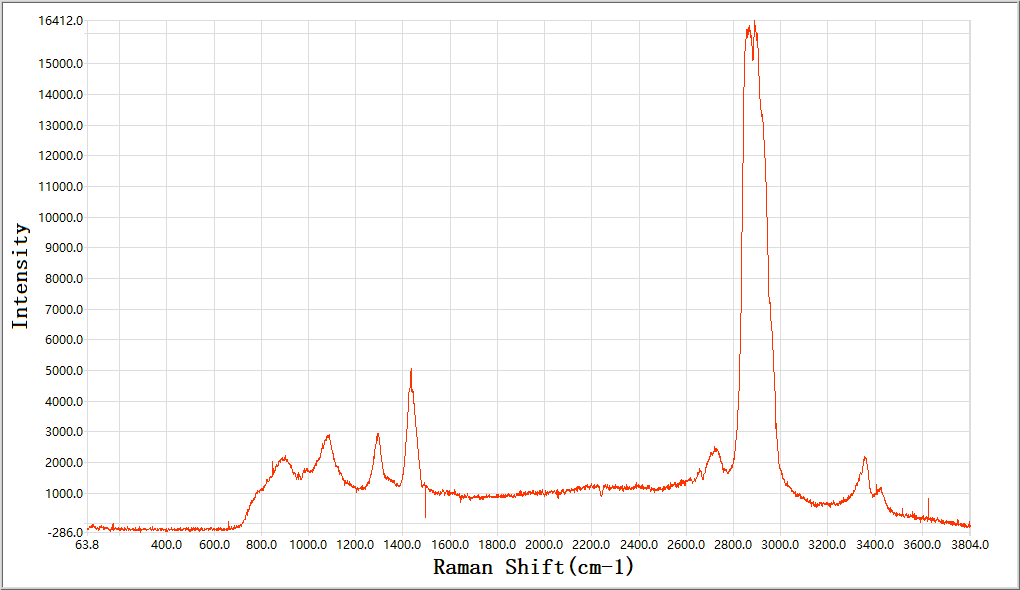
\includegraphics[width=\textwidth]{figures/己胺.png}
			\caption{1-己胺的拉曼光谱} \label{}
		\end{minipage}
	\end{figure}
	\begin{figure}[htp]
		\begin{minipage}[t]{0.5\textwidth}
			\centering
			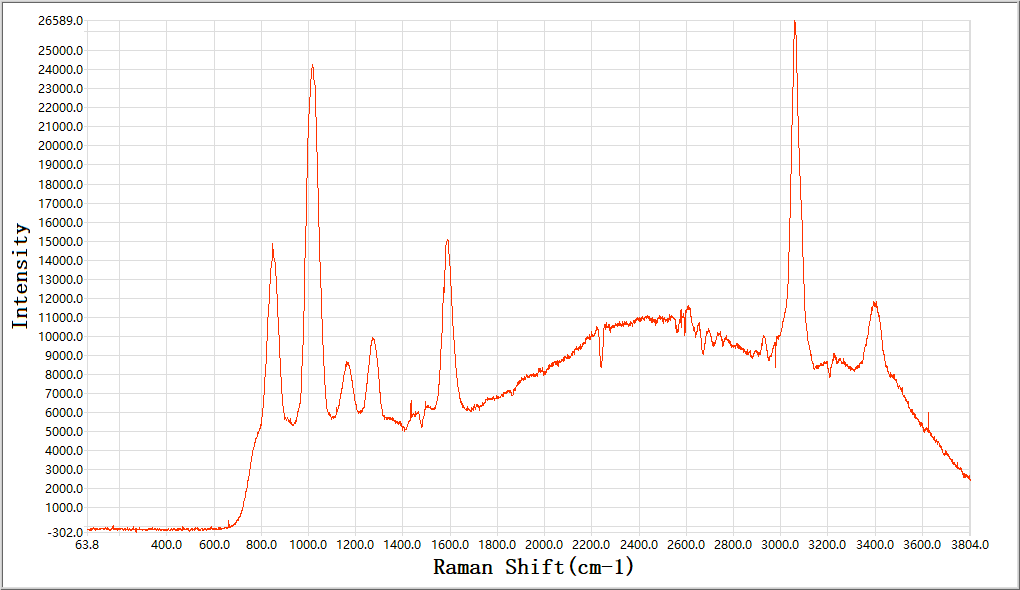
\includegraphics[width=\linewidth]{figures/苯胺.png} 
			\caption{苯胺的拉曼光谱} \label{}
		\end{minipage}
		\begin{minipage}[t]{0.5\textwidth}
			\centering
			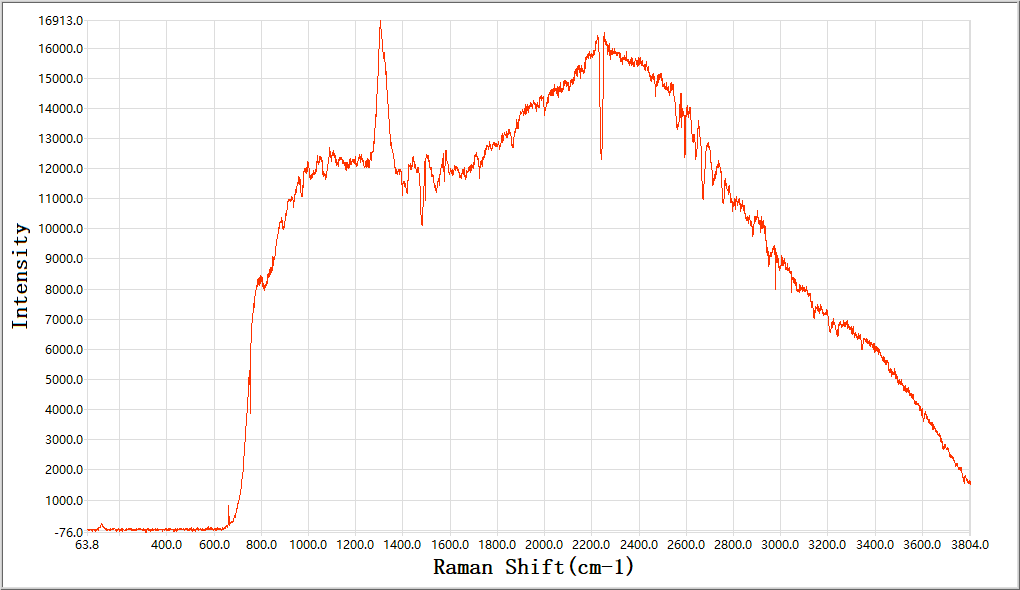
\includegraphics[width=\textwidth]{figures/对硝基苯胺.png}
			\caption{对硝基苯胺的拉曼光谱} \label{}
		\end{minipage}
	\end{figure}


	\subsection{纳米银溶胶的表面增强拉曼光谱结果展示与分析}
	增强前后对比,增强数量级说明。

	银溶胶表征。

	\subsection{水和重水混合物电解前后的拉曼光谱结果展示与分析}
	水和重水混合物电解前后的拉曼光谱如图所示。986 $\dw{cm^{-1}}$ 处的峰为硫酸钠的\ce{O-S}振动峰。2000 $\sim$ 2800 $\dw{cm^{-1}}$ 处的峰为重水的\ce{O-D}振动峰,3100 $\sim$ 3650 $\dw{cm^{-1}}$ 处的峰为水的\ce{O-H}振动峰。肉眼难以看出二者的差异,且由于水的拉曼信号较为微弱,信噪比不高,难以进行积分得到峰面积以进一步定量分析。因此采用比较振动峰高度变化的方式,电解前后的 $ I_{\ce{O-D}} / I_{\ce{O-H}}$ 分别为 10.35和11.28,因此可以认为,电解前后水的含量相对减少了 $1-10.35/11.28 \approx 8.2\%$ 。
	\begin{figure}[htp]
		\begin{minipage}[t]{0.5\textwidth}
			\centering
			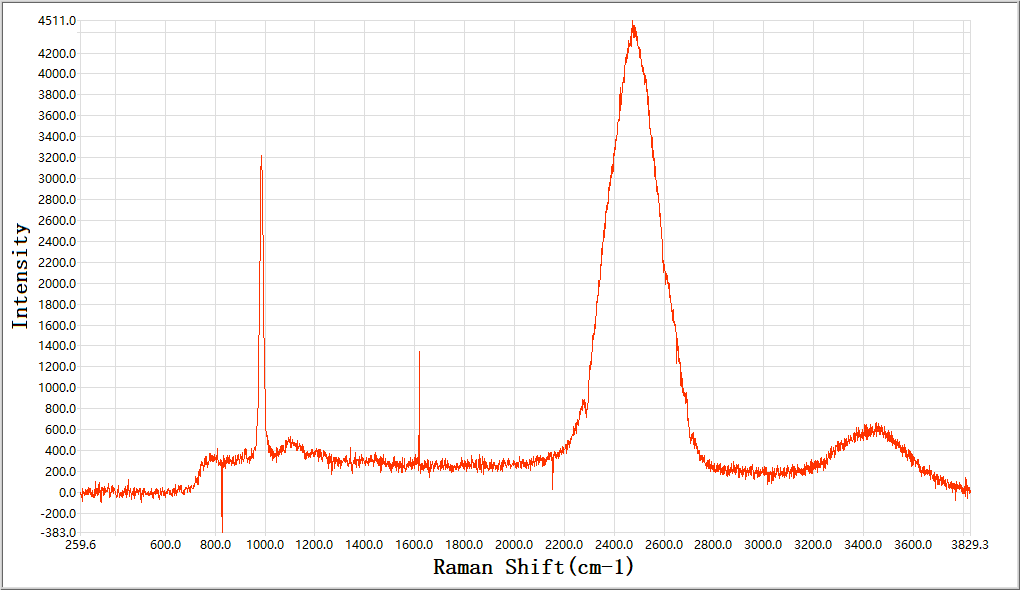
\includegraphics[width=\linewidth]{figures/电解水2.png} 
			\caption{电解前} \label{}
		\end{minipage}
		\begin{minipage}[t]{0.5\textwidth}
			\centering
			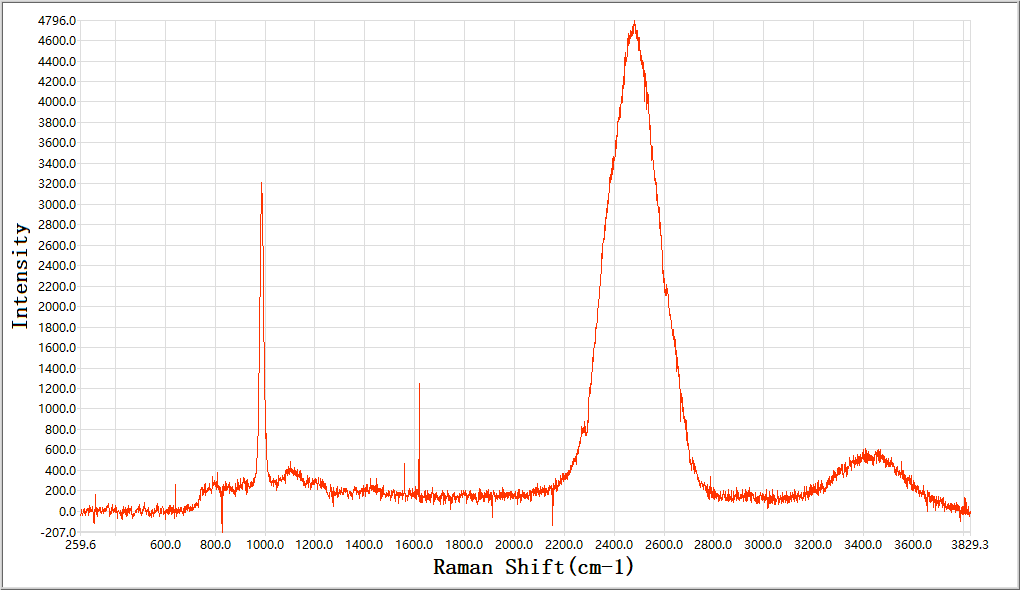
\includegraphics[width=\textwidth]{figures/电解水3.png}
			\caption{电解后} \label{}
		\end{minipage}
	\end{figure}
	
	可以根据实验条件估算上述含量变化的理论值。水在25 \dC 的密度为0.9970 g/mL,从而物质的量为22.14 mmol。电解过程转移的电子为4.66 mmol,即消耗的水为2.33 mmol,水的含量减少了 $10.5\%$,与实验结果基本一致。

	\section{结果讨论与解释}

	\subsection{纳米银溶胶的表面增强拉曼光谱效应解释}
	讨论一下表面增强的实验结果,和上面的结果展示看着各自的内容来写就行。比如如何确定有增强效果,对不同物质的增强效果。

	\subsection{水和重水混合物电解速率差异的解释}
	为进一步讨论两种羟基振动频率的变化、计算振动力学常数,取重水和水的羟基振动峰极大值位置,即分别取 $\widetilde{\nu} _{\ce{O-D}} = 2480 \dw{cm^{-1}} $ 和 $ \widetilde{\nu} _{\ce{O-H}} = 3420 \dw{cm^{-1}} $。振动的量子力学零点能为
	\begin{equation*}
		E_0 = \frac{1}{2} h \nu = \frac{1}{2} h \widetilde{\nu} c  .
	\end{equation*}
	则有 $E_{0, \ce{O-D}} = 0.154 \dw{eV}$,$E_{0, \ce{O-H}} = 0.212 \dw{eV}$。量子力学的简谐近似给出了振动频率 $\nu$ 与振动力学常数 $k$ 的关系
	\begin{gather*}
		\nu = \frac{1}{2\pi} \sqrt{\frac{k}{\mu}} ,\quad \mu = \frac{m_1 m_2}{m_1 + m_2}\,,
	\end{gather*}
	其中 $m_1, m_2$ 为化学键两个原子的质量,即
	\begin{gather*}
		k = \frac{m_1 m_2}{m_1 + m_2} (2\pi \widetilde{\nu} c)^2 \,.
	\end{gather*}
	则有$k_{\ce{O-D}} = 6.48\times 10^2 \dw{kg/s^2}$,$k_{\ce{O-H}} = 6.53\times 10^2 \dw{kg/s^2}$。二者基本一致,说明相同元素的不同同位素的化学环境非常相似。

	现在也可以解释电解过程中,水和重水电解速率的差异了。重水羟基振动的零点能,或说基态能量较水的羟基低,因此键能更大,不容易断裂,电解过程主要消耗的是水而非重水,这与上述实验与理论计算的结果相符。

	\section{结论}
	\subsection{实验小结}
	本次中级物理化学实验,我们成功搭建了一个测量范围广、信噪比高、分辨率高的拉曼光谱。同时,我们还开发了配套软件,能够方便地实时监测CCD信号,并经标定和转化得到拉曼光谱。我们借助搭建的拉曼光谱,测得了部分物质的光谱图,分析了水和重水电解速率差异与羟基振动强度的关系。我们合成了银纳米溶胶,并测试了其表面增强效果,增强了约 $10^2$ 的数量级。总的来说,我们基本达成了实验目标。

	\subsection{实验改进方向展望}
	当然,受实验课时限制,本次拉曼光谱仪项目,其实仍有不少可供继续改进之处。

	首先是仪器。本次项目中,光谱仪的性能经过多次优化,已经达到我们非常满意的程度了。不过如果死缠烂打,还有一部分的基线是可以进一步优化的,不过那就需要更多的时间、努力和耐心了。仪器的元件选择上,也有可供优化之处,例如作为教学实验提供的样品池架并不能恰好适配比色皿,这就需要测量光谱时仔细地放置比色皿以保证谱图的可重复性。但原则上这应该是仪器设计应该纳入考虑的重要因素之一。又例如,实验使用的CCD检测器,有不少像素坏点,明显干扰谱图的呈现,理论上也应该从硬件质量上规避这一问题。尽管如此,作为教学实验,最重要的还是在既有条件下,尽可能把仪器做到最好,重在仪器原理和构造实现的学习上。但如果到了课程以外,就需要更多的心思了。

	其次是软件。本次软件是借助LabView开发的,作为拉曼光谱的谱图呈现软件,标定、寻峰、谱图转换等基本功能都设计地非常完善了,大部分情况下,可以流畅使用。但其实,从软件设计专业的角度来说,这个软件还是不那么成熟的——只要使用者愿意尝试,以强烈的好奇心和欲望探索这软件的每一个按钮,总是能卡出奇奇怪怪的bug来的,换句话说,鲁棒性不足。另一方面,我们的软件其实离成熟的光谱分析软件还有不小的距离,例如实现CCD检测器信号中噪点的去除、交互式谱图的实现、积分谱图给定光谱范围、识峰、基线扣除等诸多常用的分析功能,但这也很难在半学期短短的实验课完成,更何况还是利用LabView的图形化开发界面。只能说,LabView仅供入门,难于精通。
	
	最后是基于光谱的实验设计。总的来说,时间都非常紧张,尤其是在光谱搭建已经非常耗时的情况下,从零开始摸实验条件也需要非常多的精力。一部分原因是我们小组早期的分工并不十分明确,仪器搭建、软件编写和实验准备应当一同进行才是。不过,也不能完全从事后诸葛的角度来看待,毕竟实验的前几周,我们还并没有充分的信心能够搭出一个足够好的光谱,正如我们开始准备实验时的仓促,并不知道实验的具体条件应当如何一样。在这个意义上,水和重水的电解分析,如果还有时间的话,理应可以做得更好,例如获得线性变化的关系,来进一步分析其过程。而表面增强拉曼光谱的纳米银合成和测试,同样也是非常玄学。毕竟我们虽然幸运地合成出了纳米银,也测得了表面增强效应,但纳米颗粒的粒径、形状,以及实验中起关键作用的细节,并不完全在我们的掌控之中,这也需要更加深入的原理探索。

	\section{演示视频}
	我们制作了光谱仪和软件的演示视频,可供参考。
	\begin{itemize}
		\item \url{https://www.bilibili.com/video/BV1FT411t7Rm/}
	\end{itemize}
	

	\section{致谢}
	感谢小组成员之间的通力合作,也感谢老师和助教一学期以来的指导和帮助!
	
	\section{参考文献}
	待添加,别急

	\bibliographystyle{ieeetr}
	\bibliography{reference}
	% 原生bibtex对中文支持不好,请在bibtex文献库对中文文献做以下调整:
	% 将作者以 “张三{, }李四{, }松鼠” 形式表示
	% 将版本号输入在书名一栏 例如 “物理化学实验(第四版)”


	
\end{document}